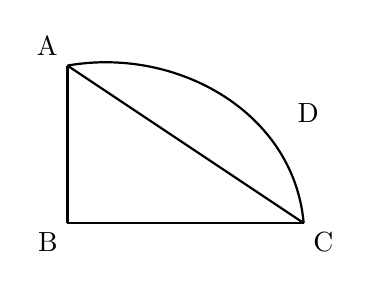
\begin{tikzpicture}[scale=1]

    % Define coordinates for the vertices based on the geometric structure
    % B is the bottom-left corner
    \coordinate (B) at (0, 0);
    % C is to the right of B
    \coordinate (C) at (3, 0);
    % A is above B, forming a right angle at B
    \coordinate (A) at (0, 2);
    
    % Draw the line segments for the triangle-like part
    \draw[thick] (A) -- (B);
    \draw[thick] (B) -- (C);
    \draw[thick] (A) -- (C);

    % Draw the arc ADC
    % This is a quarter-circle arc centered at B with radius approximately equal to segment BC
    % Start angle is 90 (at point A) and ends near 0 (at point C)
    % Note: Adjusting the arc to start from A (0,2) and end at C (3,0) implies an elliptical arc or different center
    % Based on the visual, it is an arc connecting A and C
    \draw[thick] (A) to[out=10, in=95] (3,0);

    % Place labels exactly as they appear in the image
    \node[above left] at (A) {A};
    \node[below left] at (B) {B};
    \node[below right] at (C) {C};
    \node[right] at (2.8, 1.4) {D}; % Label D is placed along the curve

\end{tikzpicture}